% ==========================================
% Section 10: Principal Component Analysis (Slides 49-51)
% ==========================================

% Slide 49: PCA Introduction
\begin{frame}{تحلیل مؤلفه‌های اصلی (\lr{PCA})}
\begin{columns}[c]
  \begin{column}{0.55\textwidth}
    \begin{itemize}
      \item \textbf{تاکنون روش‌های انتخاب ویژگی را بررسی کردیم:}
      \begin{itemize}
        \item زیرمجموعه‌ای از ویژگی‌های موجود را انتخاب می‌کردیم.
        \item هیچ ویژگی جدیدی ساخته نمی‌شد.
      \end{itemize}
      \vspace{0.3cm}
      \item \textbf{رویکرد استخراج ویژگی (\lr{Feature Extraction})}
      \begin{itemize}
        \item ترکیب ویژگی‌های موجود برای ایجاد متغیرهای جدید و متراکم.
        \item \lr{PCA (Principal Component Analysis)} محبوب‌ترین روش خطی بدون نظارت برای کاهش ابعاد است.
      \end{itemize}
    \end{itemize}
  \end{column}
  \begin{column}{0.43\textwidth}
    \centering
    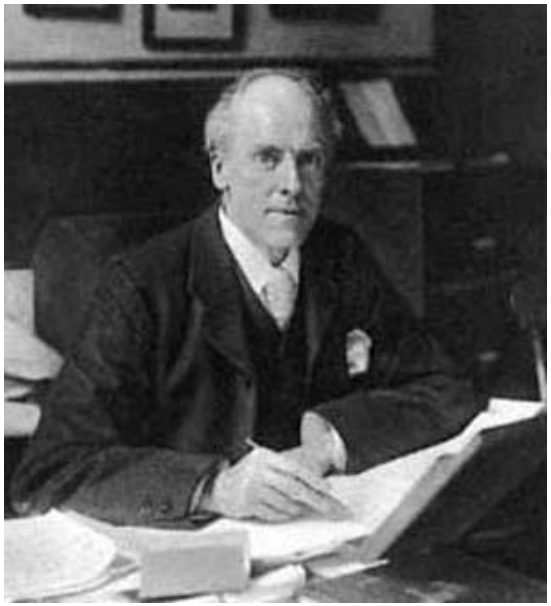
\includegraphics[width=\textwidth]{images/page_49_img_1.png}
  \end{column}
\end{columns}
\end{frame}

% Slide 50: PCA Rotation Idea
\begin{frame}{تحلیل مؤلفه‌های اصلی: ایده چرخش دستگاه مختصات}
\begin{columns}[c]
  \begin{column}{0.55\textwidth}
    \begin{itemize}
      \item \textbf{ایده بنیادین:}
      \begin{itemize}
        \item تبدیل و چرخش دستگاه مختصات به گونه‌ای که هر محور جدید (مؤلفه اصلی) در راستای بیشترین پراکندگی و واریانس داده‌ها قرار گیرد.
        \item محور اول (\lr{PC1}): بیشترین واریانس داده را جذب می‌کند.
        \item محور دوم (\lr{PC2}): متعامد بر محور اول، بیشترین واریانس باقیمانده را مدل می‌کند.
      \end{itemize}
    \end{itemize}
  \end{column}
  \begin{column}{0.43\textwidth}
    \centering
    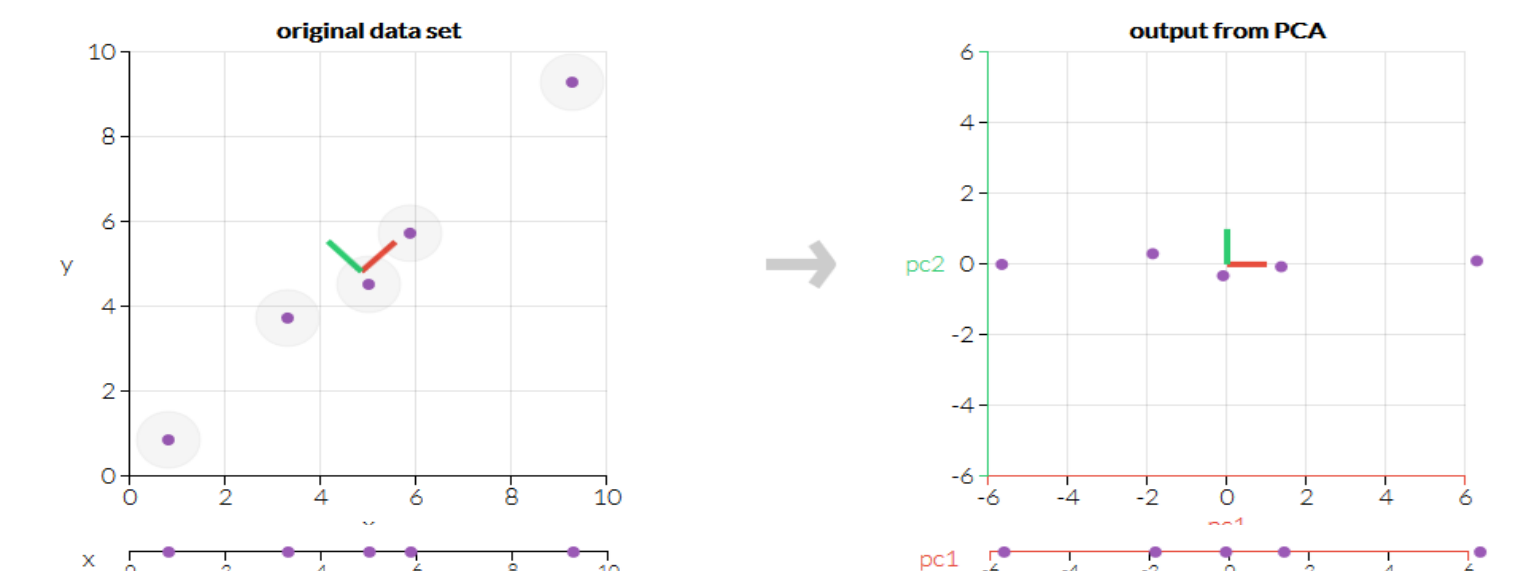
\includegraphics[width=\textwidth]{images/page_50_img_1.png}\\[8pt]
    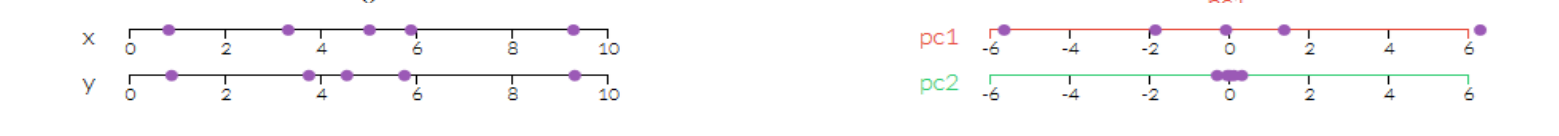
\includegraphics[width=0.9\textwidth]{images/page_50_img_2.png}
  \end{column}
\end{columns}
\end{frame}

% Slide 51: Principal Components Properties
\begin{frame}{ویژگی‌ها و کاربردهای مؤلفه‌های اصلی}
\begin{columns}[c]
  \begin{column}{0.55\textwidth}
    \begin{itemize}
      \item \textbf{مؤلفه‌های اصلی:}
      \begin{itemize}
        \item ترکیبات خطی از ویژگی‌های اولیه هستند.
        \item کاملاً ناهمبسته (\lr{Orthogonal}) با یکدیگرند.
      \end{itemize}
      \vspace{0.2cm}
      \item \textbf{رویکرد کلی در کاربرد:}
      \begin{itemize}
        \item نگه‌داشتن $k$ مؤلفه نخست به نحوی که بخش عمده واریانس داده‌ها (مثلاً \lr{95\%}) حفظ شود.
        \item کاهش فضای چندصد بعدی به ۲ یا ۳ بعد برای تجسم داده‌ها (\lr{Visualization}).
      \end{itemize}
    \end{itemize}
  \end{column}
  \begin{column}{0.43\textwidth}
    \centering
    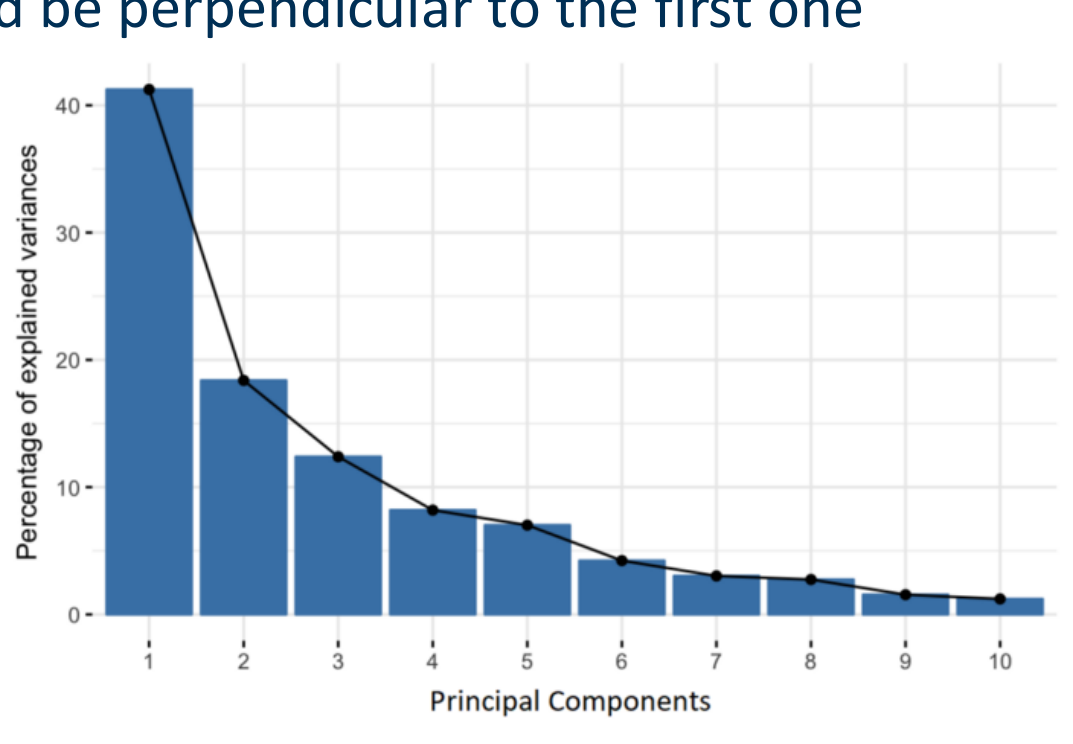
\includegraphics[width=\textwidth]{images/page_51_img_1.png}
  \end{column}
\end{columns}
\end{frame}
